% PCB vs IC Gap Diagram - v3
\documentclass[border=4mm]{standalone}
\usepackage{tikz}
\usetikzlibrary{arrows.meta, positioning, shapes.geometric, fit, calc}
\usepackage[T1]{fontenc}
\usepackage{lmodern}

% IHP Colors
\definecolor{IHPfg}{RGB}{0,80,139}
\definecolor{IHPred}{RGB}{228,15,19}
\definecolor{IHPaccent}{RGB}{109,112,114}
\definecolor{IHPlight}{RGB}{225,238,250}
\definecolor{IHPredlight}{RGB}{253,235,235}

\begin{document}
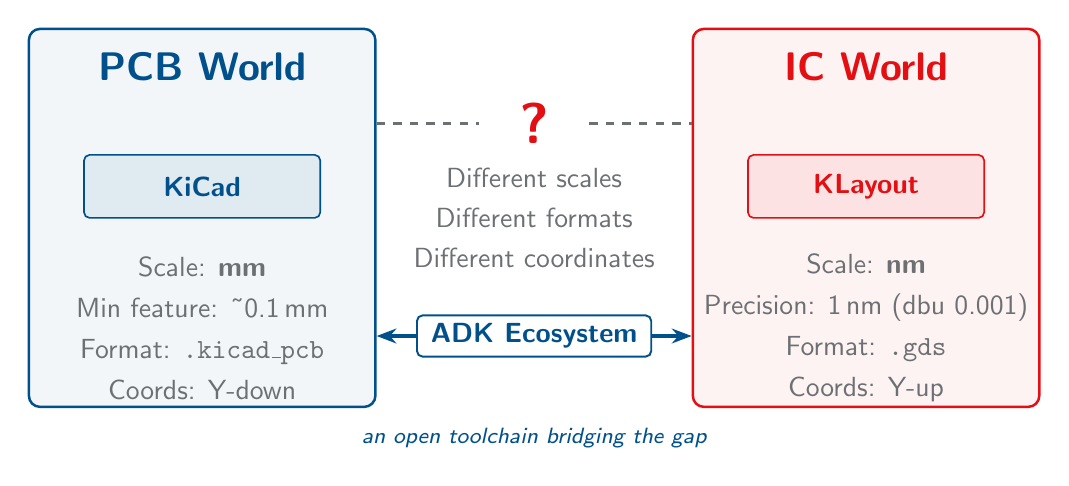
\begin{tikzpicture}[
    >=Stealth,
    worldbox/.style={
        rectangle, rounded corners=4pt,
        minimum width=44mm, minimum height=48mm,
        draw=#1, line width=0.9pt,
        fill=#1!5
    },
    worldtitle/.style={
        font=\sffamily\Large\bfseries, text=#1
    },
    toolbox/.style={
        rectangle, rounded corners=2pt,
        draw=#1, fill=#1!12, line width=0.6pt,
        minimum width=30mm, minimum height=8mm,
        font=\sffamily\normalsize\bfseries, text=#1
    },
    prop/.style={
        font=\sffamily\normalsize, text=IHPaccent, align=center
    },
    gaptext/.style={
        font=\sffamily\normalsize, text=IHPaccent, align=center
    }
]

% ---- Left: PCB World ----
\node[worldbox=IHPfg] (pcb) at (0,0) {};
\node[worldtitle=IHPfg] at ([yshift=-5mm]pcb.north) {PCB World};
\node[toolbox=IHPfg] (kicad) at ([yshift=4mm]pcb.center) {KiCad};
\node[prop] at ([yshift=-14mm]pcb.center) {
    Scale: \textbf{mm}\\[1mm]
    Min feature: \textasciitilde0.1\,mm\\[1mm]
    Format: \texttt{.kicad\_pcb}\\[1mm]
    Coords: Y-down
};

% ---- Right: IC World ----
\node[worldbox=IHPred, right=40mm of pcb] (ic) {};
\node[worldtitle=IHPred] at ([yshift=-5mm]ic.north) {IC World};
\node[toolbox=IHPred] (klayout) at ([yshift=4mm]ic.center) {KLayout};
\node[prop] at ([yshift=-14mm]ic.center) {
    Scale: \textbf{nm}\\[1mm]
    Precision: 1\,nm (dbu 0.001)\\[1mm]
    Format: \texttt{.gds}\\[1mm]
    Coords: Y-up
};

% ---- Gap (middle): the problem ----
\coordinate (gapmid) at ($(pcb.east)!0.5!(ic.west)$);

% Dashed line with "?" - positioned at top third
\draw[IHPaccent, line width=1pt, dashed]
    ([yshift=12mm]pcb.east) -- ([xshift=-7mm, yshift=12mm]gapmid);
\draw[IHPaccent, line width=1pt, dashed]
    ([xshift=7mm, yshift=12mm]gapmid) -- ([yshift=12mm]ic.west);
\node[font=\sffamily\huge\bfseries, text=IHPred] at ([yshift=12mm]gapmid) {?};

% Gap description
\node[gaptext] at (gapmid) {
    Different scales\\[0.8mm]
    Different formats\\[0.8mm]
    Different coordinates
};

% ---- Bridge: ADK Ecosystem (bottom third) ----
\draw[IHPfg, line width=1.4pt, {Stealth[length=2.5mm]}-{Stealth[length=2.5mm]}]
    ([yshift=-15mm]pcb.east) --
    node[midway, fill=white, draw=IHPfg, rounded corners=2pt,
         line width=0.7pt, inner xsep=5pt, inner ysep=3pt,
         font=\sffamily\normalsize\bfseries, text=IHPfg]
    {ADK Ecosystem}
    ([yshift=-15mm]ic.west);

\node[font=\sffamily\footnotesize\itshape, text=IHPfg]
    at ([yshift=-28mm]gapmid) {an open toolchain bridging the gap};

\end{tikzpicture}
\end{document}
